% \Chapter{}

% \chapter{RESULTADOS}

%     \section{Evaluación de la Armonización de Imágenes MSS y TM}
%         \subsection{Corrección Geométrica y Alineación Espacial}
%             La aplicación de técnicas avanzadas de corrección geométrica y alineación espacial a las imágenes MSS resultó en una mejora significativa en la precisión de su superposición con las imágenes TM. Utilizando el método LightGlue para el emparejamiento de características, se logró una reducción notable en el error de colocación, pasando de un RMSE inicial de 52.6523 a un RMSE de 0.987. Este resultado subraya la efectividad de las correcciones a nivel de píxel y subpíxel en la alineación de las imágenes, permitiendo una base sólida para la posterior armonización espectral.

%             \begin{figure}[H] 
%                 \caption{\doublespacing \\ \textit{Comparativa de Alineación: Imágenes MSS, TM y MSS Corregida.}} 
%                 \centering
%                 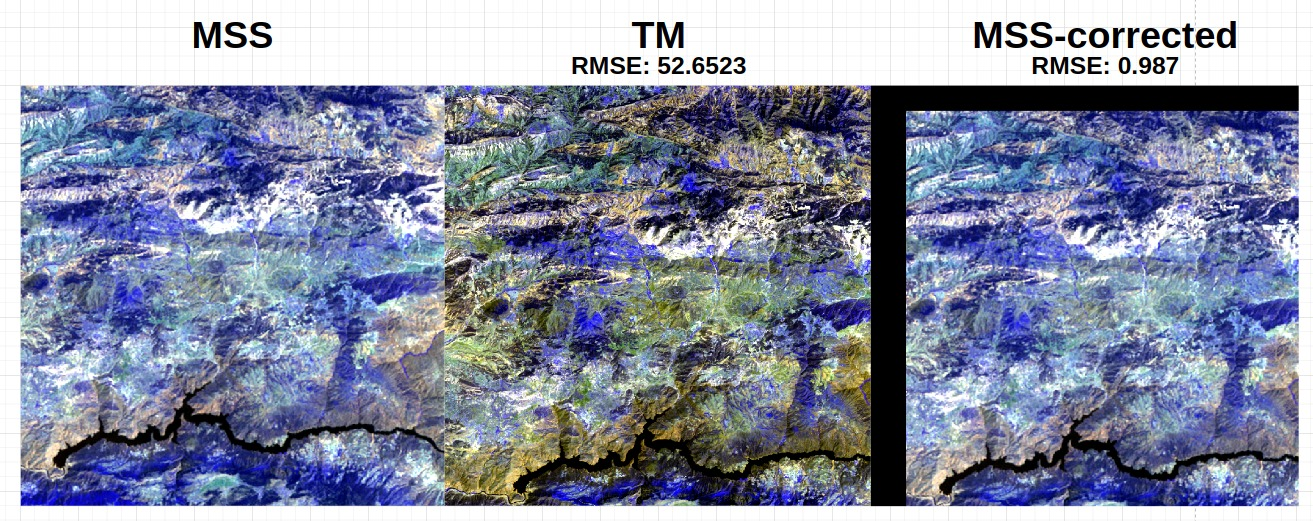
\includegraphics[width=0.8\linewidth]{2_CAPITULO0/IMG/tm_mss_rmse.png}
%                 \begin{justify}
%                     \textit{Nota.} El contraste entre la imagen MSS original y la corregida resalta con una reducción significativa del error RMSE, evidenciando la eficacia de las correcciones a nivel de píxel y subpíxel para lograr una alineación casi perfecta.
%                 \end{justify}                    
%                 \label{tm_mss_rmse}
%             \end{figure}

%         \subsection{Calidad de la Armonización Espectral y Espacial}
%             La implementación del modelo SWINIR - MSS2TM GAN mostró una capacidad excepcional para armonizar las bandas espectrales de las imágenes MSS con las correspondientes imágenes TM. 

%             \begin{figure}[H] 
%                 \caption{\doublespacing \\ \textit{Generación de bandas NIR-R-G armonizadas de MSS hacia TM.}} 
%                 \centering
%                 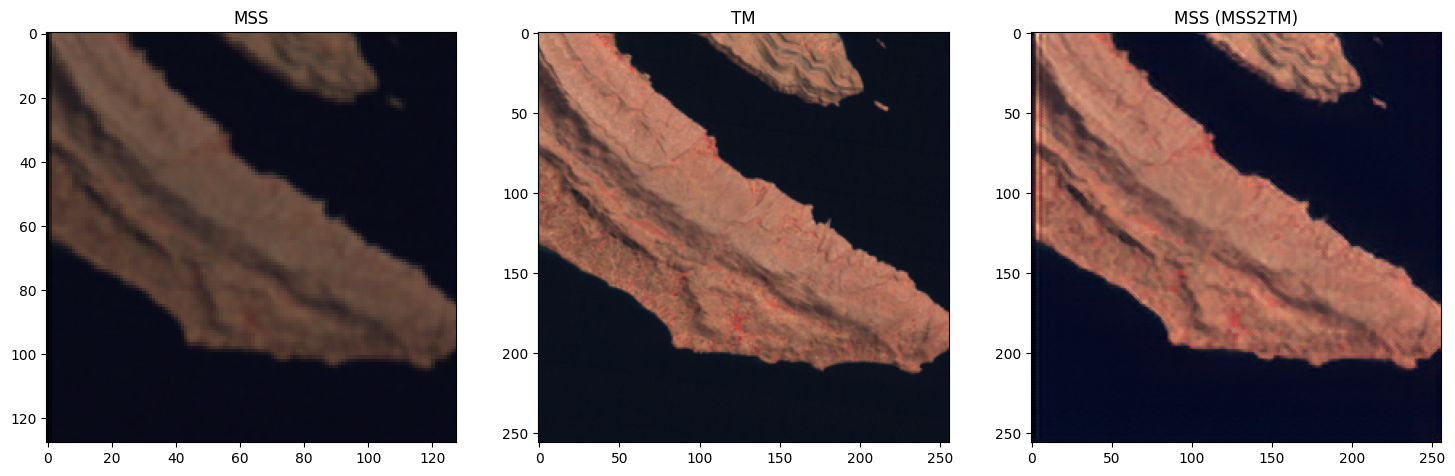
\includegraphics[width=1\linewidth]{2_CAPITULO5/IMG/espectral.png}
%                 \begin{justify}
%                     \textit{Nota.} Comparativa de imágenes MSS, TM y MSS corregida revela mejoras significativas en armonización espectral con el modelo SWINIR - MSS2TM.
%                 \end{justify}                    
%                 \label{armonizacion}
%             \end{figure}

%         \subsection{Generación de Bandas Virtuales}
%             La creación de bandas virtuales para complementar las imágenes MSS con bandas no originalmente presentes demostró ser altamente efectiva. El modelo de Perceptrón Multicapa (MLP) empleado para predecir estas bandas adicionales alcanzó una precisión de predicción con un error medio absoluto (MAE).

%             \begin{figure}[H] 
%                 \caption{\doublespacing \\ \textit{Comparación de Alineación y Generación de Bandas Virtuales.}} 
%                 \centering
%                 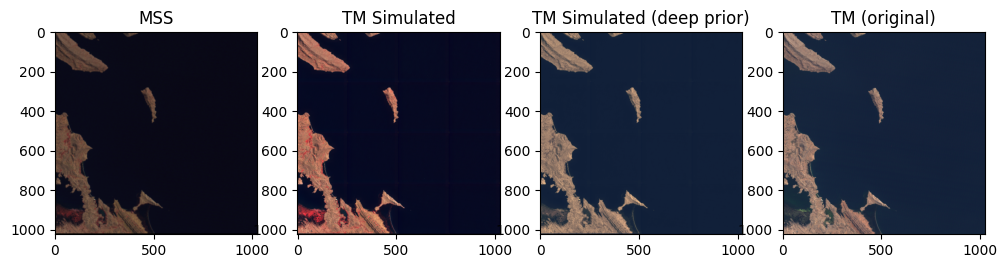
\includegraphics[width=1\linewidth]{2_CAPITULO5/IMG/bandas.png}
%                 \begin{justify}
%                     \textit{Nota.} Visualización del avance en generación de bandas virtuales MSS, mostrando la eficacia del modelo MLP en la precisión espectral frente a imágenes TM originales.
%                 \end{justify}                    
%                 \label{bandas}
%             \end{figure}
    
%     \section{Análisis Estadístico de los Resultados}
%         \subsection{Validación Cuantitativa}

%             \begin{figure}[H] 
%                 \caption{\doublespacing \\ \textit{Áreas de Validación en Perú.}} 
%                 \centering
%                 \includegraphics[width=0.6\linewidth]{2_CAPITULO5/IMG/imagenes_peru.png}
%                 \begin{justify}
%                     \textit{Nota.} Mapa de Perú mostrando puntos de muestreo para la validación de superresolución de imágenes MSS en diversas regiones geográficas.
%                 \end{justify}                    
%                 \label{modelo3}
%             \end{figure}

%             Se ha seleccionado estratégicamente el Perú como área de validación para aplicar y evaluar el proceso. La elección de esta región se debe a su variada topografía y diversidad de ecosistemas, desde la costa del Pacífico hasta las alturas de los Andes, brindando así un escenario desafiante para la superresolución satelital. Como se muestra en la imagen, se han identificado múltiples puntos distribuidos a lo largo del país, en los cuales se han extraído segmentos de imágenes MSS para su transformación a la resolución de imágenes TM.
%             La validación cuantitativa de los modelos desarrollados se realizó utilizando un conjunto de validación compuesto por 23 pares de imágenes MSS y TM. 
            

%             \begin{table}[H]
%                 \caption{\doublespacing \\ \textit{Métricas entre ímagenes simuladas y reales.}}
%                 \begin{spacing}{8}
%                     \fontsize{8pt}{2pt}\selectfont  
%                     \begin{tabularx}{\linewidth}{*{4}{X}} 
%                         \toprule
%                         \textbf{Imagen} & \textbf{MAE} & \textbf{RMSE} & \textbf{Coeficiente de Pearson} \\ 
%                         \midrule
%                         00031 & 0.2476 & 0.7194 & 0.8367 \\ 
%                         00032 & 0.2604 & 0.7465 & 0.8270 \\ 
%                         00074 & 0.2513 & 0.7089 & 0.8288 \\
%                         00213 & 0.1744 & 0.6311 & 0.9207 \\ 
%                         00273 & 0.2706 & 0.7278 & 0.8140 \\
%                         00328 & 0.1204 & 0.6364 & 0.9481 \\ 
%                         00353 & 0.2300 & 1.0631 & 0.6751 \\ 
%                         01145 & 0.2446 & 0.7009 & 0.8420 \\
%                         01440 & 0.3418 & 1.1231 & 0.6574 \\ 
%                         01465 & 0.2570 & 0.7359 & 0.8401 \\ 
%                         04590 & 0.2529 & 0.7264 & 0.8290 \\ 
%                         05720 & 0.2453 & 0.7008 & 0.8497 \\ 
%                         05883 & 0.2164 & 0.8212 & 0.8892 \\ 
%                         05826 & 0.2570 & 0.7217 & 0.8452 \\ 
%                         04706 & 0.2449 & 0.7081 & 0.8454 \\ 
%                         06008 & 0.5724 & 1.8287 & 0.2605 \\ 
%                         05935 & 0.2633 & 0.7215 & 0.8337 \\ 
%                         11030 & 0.2467 & 0.6982 & 0.8424 \\ 
%                         08849 & 0.2819 & 0.9625 & 0.7416 \\ 
%                         08927 & 0.2451 & 0.6902 & 0.8460 \\ 
%                         08929 & 0.2380 & 0.7244 & 0.8520 \\ 
%                         06776 & 0.2391 & 0.6941 & 0.8454 \\ 
%                         11281 & 0.5213 & 1.7584 & 0.2414 \\ 
%                         \bottomrule
%                     \end{tabularx}
%                 \end{spacing}
%                 \vspace{1\baselineskip}
%                 \textit{Nota.} Tabla comparativa de métricas MAE, RMSE y Pearson en superresolución de imágenes MSS por zonas, reflejando variabilidad topográfica y de respuesta del modelo.
%                 \label{valores_metricas}
%             \end{table}

%             Los valores más bajos de MAE y RMSE indican una mayor precisión en la correspondencia de las imágenes transformadas con las TM originales. El coeficiente de correlación de Pearson refleja la relación lineal entre las imágenes generadas y las de referencia, con valores más cercanos a 1 que implican una mayor correlación.

%             \begin{figure}[H] 
%                 \caption{\doublespacing \\ \textit{Distribución de Métricas de Validación.}} 
%                 \centering
%                 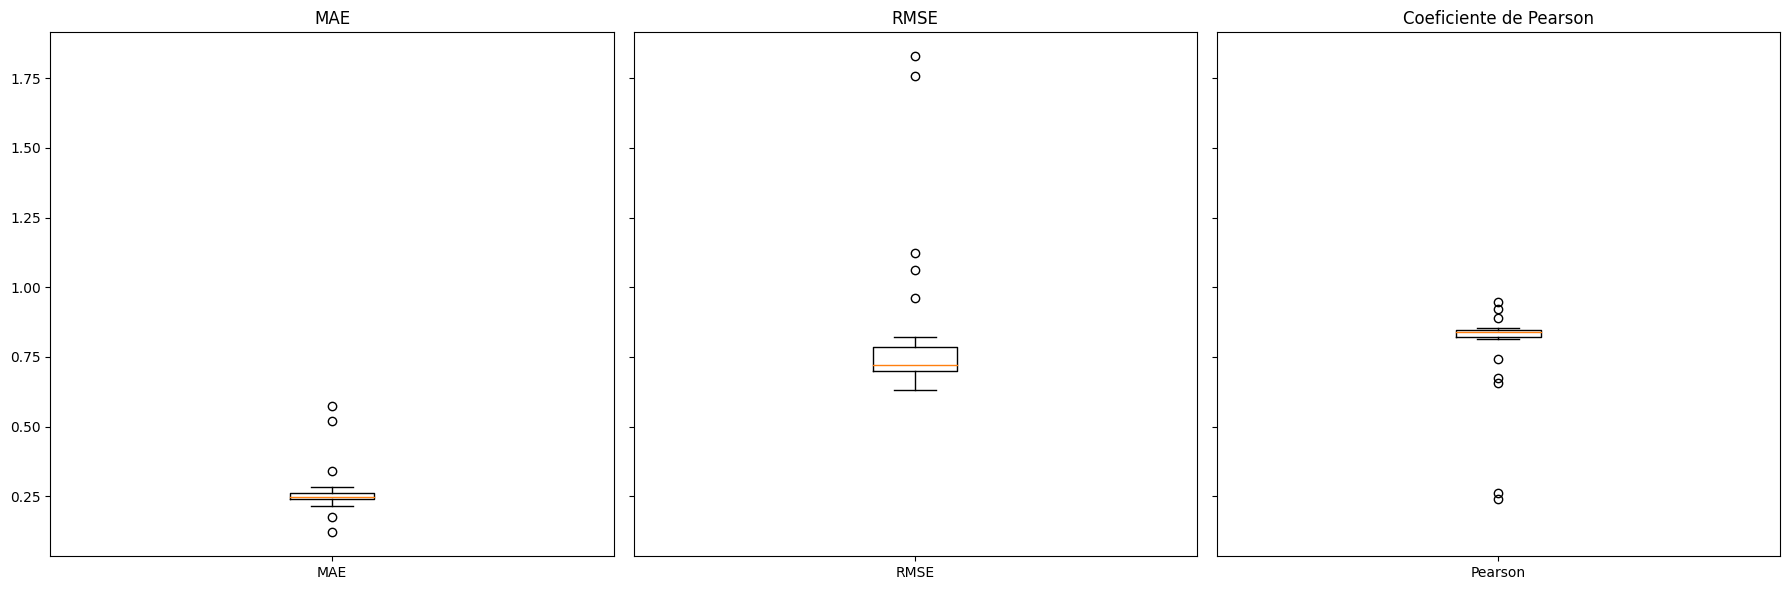
\includegraphics[width=0.9\linewidth]{2_CAPITULO5/IMG/box_plot.png}
%                 \begin{justify}
%                     \textit{Nota.} Diagrama de cajas que muestra la variabilidad y dispersión de MAE, RMSE y coeficiente de Pearson en superresolución de imágenes MSS.
%                 \end{justify}                    
%                 \label{modelo}
%             \end{figure}

%             El diagrama de cajas proporciona una visión clara de la distribución estadística de las métricas de validación aplicadas a la superresolución de imágenes MSS en Perú. Cada métrica revela aspectos distintos de la precisión del modelo MSS2TM. El MAE destaca la exactitud media en la estimación de valores de píxeles, el RMSE señala la dispersión general de los errores en las predicciones del modelo, y el coeficiente de Pearson mide la fuerza y la dirección de la relación lineal entre las imágenes generadas y las originales.

%             Los valores promedio de MAE y RMSE a lo largo de todas las imágenes evaluadas fueron 0.2710 y 0.8547, respectivamente, lo que indica un buen rendimiento general del modelo en el contexto de la superresolución. Sin embargo, hubo variabilidad en el rendimiento entre diferentes áreas, como lo demuestra el rango de valores de MAE y RMSE. La imagen identificada como 00328 mostró un desempeño sobresaliente con el MAE más bajo y el coeficiente de correlación de Pearson más alto, mientras que la imagen 06008 presentó los valores más altos de MAE y RMSE, además de la correlación más baja, lo que sugiere que ciertas áreas pueden presentar desafíos específicos para el modelo.

%             Este análisis detallado permite no solo verificar la capacidad del modelo para generar imágenes TM de alta fidelidad a partir de imágenes MSS, sino también identificar áreas donde el modelo puede requerir ajustes o entrenamiento adicional para manejar condiciones específicas del paisaje.


\Chapter{}
\chapter{PRESUPUESTO}
    \begin{table}[H]
        \caption{\doublespacing \\ \textit{Presupuesto detallado para el proyecto de investigación.}}
        \begin{spacing}{1.5}
            \fontsize{8pt}{10pt}\selectfont  
            \begin{tabularx}{\linewidth}{*{4}{P{4.5cm}}} 
                \toprule
                \multicolumn{4}{c}{\textbf{Presupuesto total (Montos aproximados en S/.)}} \\ 
                \midrule
                \textbf{Rubro} & \textbf{Costo unitario} & \textbf{Cantidad} & \textbf{Total} \\
                \midrule
                Equipos: & & & \\ 
                Laptop & 3000 & 1 & 3000 \\ 
                Disco duro de 1 Tbyte & 200 & 1 & 200 \\ 
                Internet: & & & \\ 
                Servicio de internet (12 meses) & 1400 & 1 & 1400 \\
                Papelería y útiles: & & & \\
                Materiales de escritorio & 150 & 1 & 150 \\ 
                Impresiones & 800 & 1 & 800 \\ 
                Software: & & & \\ 
                QGIS, Python, R (gratuitos) & 0 & 1 & 0 \\ 
                \midrule
                Tiempo de investigación: & & & \\
                Medio sueldo mínimo mensual & 512.5 & 12 & 6150 \\
                \midrule
                \textbf{Total General:} & & & \textbf{11700} \\
                \bottomrule
            \end{tabularx}
        \end{spacing}
        \vspace{1\baselineskip}
        \textit{Nota.} El presupuesto incluye equipamiento, servicios, materiales y el costo estimado del tiempo del investigador basado en medio sueldo mínimo mensual, reflejando la dedicación parcial al proyecto durante un año. No incluye otros posibles gastos indirectos o costos de oportunidad.
        \label{Presupuesto}
    \end{table}

